\chapter{Mecánica Hamiltoniana} 
\section{Transformada de Legendre} \refstepcounter{subsection}
Si consideramos una función de una variable $y=f(x)$ tal que $f''(x)\neq 0$, entonces a cada punto le corresponde una sola recta tangente asociada, asociada con su pendiente $f'(x)$ y su ordenada en el origen $g$, tal que $y = f'(x)x + g$, a esta familia de rectas definida por el par $(f'(x),g)$ se le llama \textbf{envolvente} y contiene toda la información original de la función.
\begin{marginfigure}[0cm]
	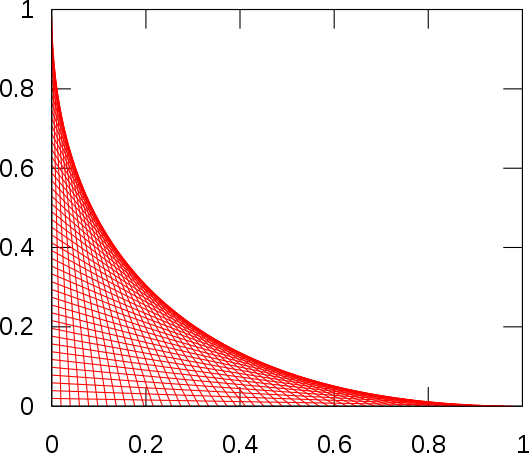
\includegraphics{envelope.png}
	\labfig{margin1}
\end{marginfigure}
Así tenemos dos nuevas coordenadas $[p,g(p)]$, relacionadas con $[x,f(x)]$ mediante
\vspace{-15pt}
\begin{equation} \label{4.1.1}
    \begin{matrix}
        p(x)=f'(x) && \color{blue}g(p)\color{black}=f(x(p))-x(p)\color{blue}p\color{black} &&[x,f(x)] \mapsto [p,g(p)] \\
        x(p)=(f')^{-1}(p) &&  \color{blue}f(x) \color{black}=p(x)\color{blue}x\color{black}+g(p(x))  && [p,g(p)] \mapsto [x,f(x)]\
    \end{matrix}
\end{equation} \refstepcounter{subsection}
Donde la primera expresión es la \textit{Transformada de Legendre}, y será invertible (la segunda expresión) siempre que $f'(x)$ sea invertible (cierto si $f''(x)\neq 0$).
\subsection{Varias variables}
Si ahora tenemos $f(\{x_i,y_i\})$ donde $\{y_i\}$ son las variables sobre las que queremos hacer la transformada, la transformada es entonces
\begin{equation} \label{4.1.2}
    \begin{matrix}
        p_i(\{x_i,y_i\})=\frac{\partial f}{\partial y_i} && g(\{x_i,\color{blue}p_i\color{black}\}) =f(\{x_i,p_i\}) -\sum_j \color{blue}p_j\color{black} y_j(\{x_i,p_i\})  &&[y_i,f(\{x_i,y_i\})] \mapsto [p_i,g(\{x_i,p_y\})] \\
        y_i(\{x_i,p_i\})=\left[\frac{\partial f}{\partial y_i}\right]^{-1} && f(\{x_i,\color{blue}y_i\color{black}\}) =\sum_j \color{blue}y_j\color{black} p_j (\{x_i,y_i\})  +g(\{x_i,y_i\}) &&[p_i,g(\{x_i,y_i\})] \mapsto [y_i,f(\{x_i,y_i\})]\\
    \end{matrix}
\end{equation} \refstepcounter{subsection}
La transformación será inversible si el jacobiano de $y_i \mapsto p_i$ es no nulo.
\subsubsection{Transformada de Legendre del Lagrangiano}
Ahora si tenemos $\pazocal{L}(\{q_j,\dot{q}_j\};t)$, $\{\dot{q}_j\}$ serán nuestras antiguas variables y las nuevas variables serán $\partial_{\dot{q}_j}\pazocal{L}=p_j$, los momentos generalizados o conjugados. Entonces aplicando (4.1.2) llegamos a (3.1.2)
\begin{equation} \label{4.1.3}
        p_i(\{q_i,\dot{q}_i\};t)=\frac{\partial \pazocal{L}}{\partial q_i} \ \ \ \ \ \  g(\{q_i,p_i\};t) =\pazocal{L}(\{q_i,p_i\};t) -\sum_j^s \dot{q}_j p_j(\{q_i,p_i\}) = -\pazocal{H}
\end{equation} \refstepcounter{subsection}
De esta forma, $\pazocal{H}$ es equivalente a la \textit{Transformada de Legendre} de $\pazocal{L}$ con respecto a los $\dot{q}_j$, y esta es inversible, la demostración de que el jacobiano de $[\partial_{\dot{q}_j}p_i]$ es no nulo bajo ciertas circumstancias es *añadir*.

De esta forma, no hemos perdido ninguna información del sistema al pasar de $\pazocal{L}$ a $\pazocal{H}$, y a continuación reformularemos las ecuaciones del movimiento en función de esta cantidad de una forma equivalente a la fomulación lagrangiana.
\section{Ecuaciones de Hamilton} \refstepcounter{subsection}
Si hacemos la diferencial exacta de $\pazocal{H}$ usando la regla de la cadena tenemos
\begin{equation} \label{4.2.1}
    d\pazocal{H} = \sum^s\left(\frac{\partial \pazocal{H}}{\partial q_j}dq_j+\frac{\partial \pazocal{H}}{\partial p_j}dp_j\right)+\frac{\partial \pazocal{H}}{\partial t} dt
\end{equation} \refstepcounter{subsection}
Si por otro lado hacemos el diferencial de $\pazocal{H}$ desde (3.1.2) o (4.1.3)
\begin{equation} \label{4.2.2}
    d\pazocal{H} = \sum^s\left(p_j dq_j+\dot{q}_j dp_j\right)-dL
\end{equation} \refstepcounter{subsection}
si $d\pazocal{L}$ es por regla de la cadena, y usando (2.2.1) y (2.2.2)
\begin{equation} \label{4.2.3}
    d\pazocal{L}= \sum^s\left(\frac{\partial \pazocal{L}}{\partial q_j}dq_j+\frac{\partial \pazocal{L}}{\partial \dot{q}_j}d\dot{q}_j\right) + \frac{\partial \pazocal{L}}{\partial t}dt = \sum^s\left(\dot{p}_j dq_j+p_j d\dot{q}\right) + \frac{\partial \pazocal{L}}{\partial t}dt
\end{equation} \refstepcounter{subsection}
Sustituyendo (4.2.3) en (4.2.2)
\begin{equation} \label{4.2.4}
    d\pazocal{H} = \sum^s p_j dq_j+\dot{q}_j dp_j-\sum^s \dot{p}_j dq_j+p_j d\dot{q}_j - \frac{\partial \pazocal{L}}{\partial t}dt = \sum^s \dot{q}_j dq_j-\dot{p}_j dq_j - \frac{\partial \pazocal{L}}{\partial t}dt
\end{equation} \refstepcounter{subsection}
Como $dq_j$, $dp_j$ y $dt$ son funciones independientes y arbitrarias, podemos igualar término a término (4.2.4) y (4.2.1), de tal forma que obtenemos tres ecuaciones
\Large \begin{equation} \label{4.2.5}
    \boxed{\dot{q}_j = \frac{\partial \pazocal{H}}{\partial p_j} \ \ \ \ \ \ \dot{p}_j= -\frac{\partial \pazocal{H}}{\partial q_j}}
\end{equation} \refstepcounter{subsection} \normalsize
Estas dos primeras ecuaciones son las \textit{Ecuaciones de Hamilton} del movimiento o \textit{Ecuaciones canónicas}. Por otro lado tenemos la tercera ecuación, que junto a (3.1.2)
\begin{equation} \label{4.2.6}
    \frac{\partial \pazocal{H}}{\partial t} = - \frac{\partial \pazocal{L}}{\partial t} = \frac{d \pazocal{H}}{dt}
\end{equation} \refstepcounter{subsection}
De esta forma, si $\pazocal{H}$ no depende explícitamente del tiempo, este se conserva.

Para aplicar estas ecuaciones en un sistema holonómico tenemos que hayar primero $\pazocal{L}$, tras esto hayar los momentos generalizados y despues invertir la relación, tal que
\begin{equation} \label{4.2.7}
    p_j = \frac{\partial \pazocal{L}}{\partial \dot{q}_j}=p_j(\{q_k,\dot{q}_k\};t)} \rightarrow \dot{q}_j = \dot{q}_j(\{q_k,p_k\};t)
\end{equation} \refstepcounter{subsection}
Entonces usamos la ecuación (4.1.3) con mucho cuidado de reemplazar todas las $\dot{q}_j$ por (4.2.7), y ya tendremos $\pazocal{H}$ en una forma que nos permita resolverlo usando (4.2.5).
\subsubsection{Ejemplo}
Un ejemplo sencillo es el péndulo simple donde $\pazocal{L}=1/2ml¹\dot{\theta}^2+mgl\cos{\theta}$, hallamos $p_\theta = \partial_\theta \pazocal{L}=ml^2\dot{\theta}$, entonces despejamos $\dot{\theta}=p_\theta/ml^2=\dot{\theta}(p_\theta).$ Sustituyendo tenemos $\pazocal{H}=p_\theta \dot{\theta} -\pazocal{L}=p_\theta^2/ml^2 - p_\theta^2/2ml^2-mgl\cos\theta = p_\theta^2/2ml^2-mgl\cos\theta = T+U$.

Ahora aplicamos (4.2.5), tal que $\dot{\theta} = p_\theta/ml^2$ para la primera, de donde sacamos que $\dot{p}_\theta=ml^2 \ddot{\theta}$ y la segunda $\dot{p}_\theta=-mgl\sin\theta$, igualando y depejando obtnemos $\ddot{\theta} + g/l \sin\theta = 0$.

La formulación Lagrangiana es mejor para tratar con ligaduras, pero la hamiltoniana nos permite reducir el orden de la ecuación diferencial resultante cuando una o varias coordenadas generalizadas son ignorables, puesto que en (3.1.5) todavía tenemos que resolver las $\dot{q}$ detro del $p$, solo conseguimos reducir en 1 el orden de un ecuación de E-L, mientras que en la formulación hamiltoniana, si una variable es cíclica, es decir $\partial_{q_j}\pazocal{H} \iff $ ignorable por (4.2.5.B), entonces ya hemos resuelto $p_j=\alpha$, y entonces podemos resolver el resto de ecuaciones, $2s-2$ y luego resolver (4.2.5.A) integrando pues es sepatable ya que $\pazocal{H}$ no depende de $q_j$ y $p_j$ es una constante.